\documentclass[10pt,aspectratio=169,serif]{beamer}

\usepackage[fontset=none, scheme=plain]{ctex}
\IfFontExistsTF{Songti SC}{%
	\setCJKmainfont{Songti SC}[AutoFakeSlant=0.2]%
	\setCJKsansfont{Songti SC}[AutoFakeSlant=0.2]%
}{%
	\setCJKmainfont{FandolSong-Regular}[Extension=.otf,BoldFont=FandolSong-Bold,AutoFakeSlant=0.2]%
	\setCJKsansfont{FandolSong-Regular}[Extension=.otf,BoldFont=FandolSong-Bold]%
}
\usepackage{amsmath,amssymb,graphicx,tikz,booktabs,multicol,calligra}
\usepackage{pgfplots}
\pgfplotsset{compat=1.18}
\usepackage{tcolorbox}
\tcbuselibrary{skins}
\usepackage{XyygU}
\usepackage{caption}
\captionsetup[figure]{name=图,labelsep=period}

\usetikzlibrary{arrows.meta,positioning,calc}

\setlength{\abovedisplayskip}{0pt plus 2pt minus 2pt}
\setlength{\belowdisplayskip}{0pt plus 2pt minus 2pt}

\title[复习参考题5]{复习参考题 5：三角函数}
\subtitle{复习巩固 \& 综合运用 \& 拓广探索}
\author{}
\institute{}
\date{2026-10-16}

\begin{document}

\begin{frame}
  \titlepage
\end{frame}

\begin{frame}{第一部分：复习巩固（第1--15题）}
\end{frame}

% --- 1 ---
\begin{frame}[t]{第1题：终边相同的角}
\textbf{1.} 写出与下列各角终边相同的角的集合 $S$，并把 $S$ 中适合 $-2\pi\le\beta<4\pi$ 的元素 $\beta$ 写出来：
\begin{enumerate}
  \item $\dfrac{\pi}{4}$；\quad
  \item $-\dfrac23\pi$；\quad
  \item $\dfrac{12}{5}\pi$；\quad
  \item $0$。
\end{enumerate}
\end{frame}

\begin{frame}[t]{第1题 解答}
\begin{tcolorbox}[colback=orange!10,colframe=orange,title=\textbf{解}]
(1) $S=\{\beta\mid\beta=\dfrac{\pi}{4}+2k\pi,\ k\in\mathbf{Z}\}$。在 $[-2\pi,4\pi)$ 内：$-\dfrac{7\pi}{4},\dfrac{\pi}{4},\dfrac{9\pi}{4}$。

(2) $S=\{\beta\mid\beta=-\dfrac{2\pi}{3}+2k\pi\}$。范围内：$-\dfrac{2\pi}{3},\dfrac{4\pi}{3},\dfrac{10\pi}{3}$。

(3) $\dfrac{12\pi}{5}=2\pi+\dfrac{2\pi}{5}$，$S=\{\beta\mid\beta=\dfrac{2\pi}{5}+2k\pi\}$。范围内：$-\dfrac{8\pi}{5},\dfrac{2\pi}{5},\dfrac{12\pi}{5}$。

(4) $S=\{\beta\mid\beta=2k\pi\}$。范围内：$-2\pi,0,2\pi$。
\end{tcolorbox}
\end{frame}

% --- 2 ---
\begin{frame}[t]{第2题：扇形弧长与面积}
\textbf{2.} 一个扇形的弧长与面积的数值都是 $5$，求这个扇形中心角的度数（精确到 $1^\circ$）。
\end{frame}

\begin{frame}[t]{第2题 解答}
\begin{tcolorbox}[colback=orange!10,colframe=orange,title=\textbf{解}]
设半径 $r$，中心角 $\alpha$（弧度）。弧长 $l=r\alpha=5$，面积 $S=\dfrac12 r^2\alpha=5$。
由 $r\alpha=5$ 得 $r=\dfrac{5}{\alpha}$，代入面积：
\[
\frac12\cdot\frac{25}{\alpha^2}\cdot\alpha=5\ \Longrightarrow\ \frac{25}{2\alpha}=5\ \Longrightarrow\ \alpha=\frac52=2.5\ \text{rad}.
\]
换算：$2.5\times\dfrac{180^\circ}{\pi}\approx 143^\circ$。
\end{tcolorbox}
\end{frame}

% --- 3 ---
\begin{frame}[t]{第3题：已知一个三角函数值求其余}
\textbf{3.}
\begin{enumerate}
  \item 已知 $\cos\varphi=\dfrac14$，求 $\sin\varphi$，$\tan\varphi$。
  \item 已知 $\sin x=2\cos x$，求角 $x$ 的三个三角函数值。
\end{enumerate}
\end{frame}

\begin{frame}[t]{第3题 解答}
\begin{tcolorbox}[colback=orange!10,colframe=orange,title=\textbf{解}]
(1) $\sin^2\varphi=1-\dfrac1{16}=\dfrac{15}{16}$。$\varphi$ 象限未定：
若 $\varphi$ 在第一、二象限，$\sin\varphi=\dfrac{\sqrt{15}}{4}$，$\tan\varphi=\sqrt{15}$；
若 $\varphi$ 在第三、四象限，$\sin\varphi=-\dfrac{\sqrt{15}}{4}$，$\tan\varphi=-\sqrt{15}$。

(2) $\sin x=2\cos x\Rightarrow\tan x=2$。由 $1+\tan^2 x=\sec^2 x$，$\cos^2 x=\dfrac15$。
若 $x$ 在一、四象限：$\cos x=\dfrac{\sqrt5}{5}$，$\sin x=\dfrac{2\sqrt5}{5}$，$\tan x=2$；
若 $x$ 在二、三象限：$\cos x=-\dfrac{\sqrt5}{5}$，$\sin x=-\dfrac{2\sqrt5}{5}$，$\tan x=2$。
\end{tcolorbox}
\end{frame}

% --- 4 ---
\begin{frame}[t]{第4题：由 $\tan\alpha=-\frac13$ 计算}
\textbf{4.} 已知 $\tan\alpha=-\dfrac13$，计算：
\begin{multicols}{2}
\begin{enumerate}
  \item $\dfrac{\sin\alpha+2\cos\alpha}{5\cos\alpha-\sin\alpha}$；
  \item $\dfrac{1}{2\sin\alpha\cos\alpha+\cos^2\alpha}$；
  \item $\sin\alpha\cos\alpha$；
  \item $(\sin\alpha+\cos\alpha)^2$。
\end{enumerate}
\end{multicols}
\end{frame}

\begin{frame}[t]{第4题 解答}
\begin{tcolorbox}[colback=orange!10,colframe=orange,title=\textbf{解}]
由 $\tan\alpha=-\dfrac13$，$\sin\alpha\cos\alpha=\dfrac{\tan\alpha}{1+\tan^2\alpha}=\dfrac{-1/3}{1+1/9}=-\dfrac{3}{10}$。

(1) 分子分母同除 $\cos\alpha$：$\dfrac{\tan\alpha+2}{5-\tan\alpha}=\dfrac{-1/3+2}{5+1/3}=\dfrac{5/3}{16/3}=\dfrac{5}{16}$。

(2) 分母 $=\cos^2\alpha(2\tan\alpha+1)=\dfrac{1}{1+\tan^2\alpha}(2\cdot(-1/3)+1)=\dfrac{9}{10}\cdot\dfrac13=\dfrac{3}{10}$。原式 $=\dfrac{10}{3}$。

(3) $\sin\alpha\cos\alpha=-\dfrac{3}{10}$。

(4) $=1+2\sin\alpha\cos\alpha=1-\dfrac{3}{5}=\dfrac{2}{5}$。
\end{tcolorbox}
\end{frame}

% --- 5 ---
\begin{frame}[t]{第5题：求三角函数值}
\textbf{5.} 计算（可用计算工具，第(2)(3)题精确到 $0.0001$）：
\begin{enumerate}
  \item $\sin\dfrac{25\pi}{6}+\cos\dfrac{25\pi}{3}+\tan\!\left(-\dfrac{25\pi}{4}\right)$；
  \item $\sin 2+\cos 3+\tan 4$；
  \item $\cos(\sin 2)$。
\end{enumerate}
\end{frame}

\begin{frame}[t]{第5题 解答}
\begin{tcolorbox}[colback=orange!10,colframe=orange,title=\textbf{解}]
(1) 利用周期性：$\dfrac{25\pi}{6}=4\pi+\dfrac{\pi}{6}$，$\dfrac{25\pi}{3}=8\pi+\dfrac{\pi}{3}$，$-\dfrac{25\pi}{4}=-6\pi-\dfrac{\pi}{4}$。
原式 $=\sin\dfrac{\pi}{6}+\cos\dfrac{\pi}{3}+\tan\!\left(-\dfrac{\pi}{4}\right)=\dfrac12+\dfrac12-1=0$。

(2) $\sin 2\approx 0.9093$，$\cos 3\approx -0.98999$，$\tan 4\approx 1.1578$。
和 $\approx 0.9093-0.9900+1.1578=1.0771$。

(3) $\sin 2\approx 0.9093$，$\cos(0.9093)\approx 0.6144$。
\end{tcolorbox}
\end{frame}

% --- 6 ---
\begin{frame}[t]{第6题：填表（$\pi<x<2\pi$）}
\textbf{6.} 设 $\pi<x<2\pi$，填表：
\begin{center}
\begin{tabular}{|c|c|c|c|c|c|c|}
\hline
$x$ & $\frac{7\pi}{6}$ &  &  &  & $\frac{7\pi}{4}$ & \\
\hline
$\sin x$ &  &  &  & $-1$ &  & \\
\hline
$\cos x$ &  & $-\frac{\sqrt2}{2}$ &  &  &  & $\frac{\sqrt3}{2}$ \\
\hline
$\tan x$ &  &  & $\sqrt3$ &  &  & \\
\hline
\end{tabular}
\end{center}
\end{frame}

\begin{frame}[t]{第6题 解答}
\begin{tcolorbox}[colback=orange!10,colframe=orange,title=\textbf{解}]
\begin{tabular}{l|cccccc}
$x$ & $\frac{7\pi}{6}$ & $\frac{5\pi}{4}$ & $\frac{4\pi}{3}$ & $\frac{3\pi}{2}$ & $\frac{7\pi}{4}$ & $\frac{11\pi}{6}$\\
\hline
$\sin x$ & $-\frac12$ & $-\frac{\sqrt2}{2}$ & $-\frac{\sqrt3}{2}$ & $-1$ & $-\frac{\sqrt2}{2}$ & $-\frac12$\\
$\cos x$ & $-\frac{\sqrt3}{2}$ & $-\frac{\sqrt2}{2}$ & $-\frac12$ & $0$ & $\frac{\sqrt2}{2}$ & $\frac{\sqrt3}{2}$\\
$\tan x$ & $\frac{\sqrt3}{3}$ & $1$ & $\sqrt3$ & 不存在 & $-1$ & $-\frac{\sqrt3}{3}$
\end{tabular}
\end{tcolorbox}
\end{frame}

% --- 7 ---
\begin{frame}[t]{第7题：最大最小值}
\textbf{7.} 求下列函数的最大值、最小值，并求使函数取得最大、最小值的 $x$ 的集合：
\begin{enumerate}
  \item $y=\sqrt2+\dfrac{\sin x}{\pi}$；\qquad
  \item $y=3-2\cos x$。
\end{enumerate}
\end{frame}

\begin{frame}[t]{第7题 解答}
\begin{tcolorbox}[colback=orange!10,colframe=orange,title=\textbf{解}]
(1) $\sin x\in[-1,1]$，故 $y_{\max}=\sqrt2+\dfrac1\pi$（$x=\dfrac{\pi}{2}+2k\pi$），$y_{\min}=\sqrt2-\dfrac1\pi$（$x=\dfrac{3\pi}{2}+2k\pi$）。

(2) $\cos x\in[-1,1]$，$y_{\max}=3+2=5$（$x=\pi+2k\pi$），$y_{\min}=3-2=1$（$x=2k\pi$）。
\end{tcolorbox}
\end{frame}

% --- 8 ---
\begin{frame}[t]{第8题：由 $y=\sin x$ 变换}
\textbf{8.} 画出下列函数在长度为一个周期的闭区间上的简图，并指出分别由 $y=\sin x,\ x\in\mathbf{R}$ 的图象经过怎样的变换得到：
\begin{enumerate}
  \item $y=\dfrac12\sin\!\left(3x-\dfrac{\pi}{3}\right)$；
  \item $y=-2\sin\!\left(x+\dfrac{\pi}{4}\right)$；
  \item $y=1-\sin\!\left(2x-\dfrac{\pi}{5}\right)$；
  \item $y=3\sin\!\left(\dfrac{\pi}{6}-\dfrac{x}{3}\right)$。
\end{enumerate}
\end{frame}

\begin{frame}[t]{第8题 解答}
\begin{tcolorbox}[colback=orange!10,colframe=orange,title=\textbf{解}]
(1) 右移 $\dfrac{\pi}{3}$，横坐标缩到 $\dfrac13$，纵坐标缩到 $\dfrac12$。$A=\dfrac12,T=\dfrac{2\pi}{3}$。

(2) 左移 $\dfrac{\pi}{4}$，纵坐标伸长到 $2$ 倍并关于 $x$ 轴翻转。$A=2,T=2\pi$。

(3) 右移 $\dfrac{\pi}{5}$，横坐标缩到 $\dfrac12$，关于 $x$ 轴翻转，再上移 $1$。$A=1,T=\pi$，值域 $[0,2]$。

(4) $y=3\sin\!\left(\dfrac{\pi}{6}-\dfrac{x}{3}\right)=-3\sin\!\left(\dfrac{x}{3}-\dfrac{\pi}{6}\right)$。右移 $\dfrac{\pi}{2}$，横坐标伸长到 $3$ 倍，纵坐标伸长到 $3$ 倍并翻转。$A=3,T=6\pi$。
\end{tcolorbox}
\end{frame}

% --- 9 ---
\begin{frame}[t]{第9题：描点法与扩展}
\textbf{9.}
\begin{enumerate}
  \item 用描点法画出函数 $y=\sin x$，$x\in\left[0,\dfrac{\pi}{2}\right]$ 的图象；
  \item 如何根据第(1)小题并运用正弦函数的性质，得到 $y=\sin x$，$x\in[0,2\pi]$ 的图象？
  \item 如何根据第(2)小题并通过平行移动坐标轴，得到 $y=\sin(x+\varphi)+k$，$x\in[0,2\pi]$ 的图象？
\end{enumerate}
\end{frame}

\begin{frame}[t]{第9题 解答}
\begin{tcolorbox}[colback=orange!10,colframe=orange,title=\textbf{解}]
(1) 取 $(0,0),(\frac{\pi}{6},\frac12),(\frac{\pi}{4},\frac{\sqrt2}{2}),(\frac{\pi}{3},\frac{\sqrt3}{2}),(\frac{\pi}{2},1)$ 描点连线。

(2) 由 $\sin(\pi-x)=\sin x$，得到 $[\frac{\pi}{2},\pi]$ 上图象与 $[0,\frac{\pi}{2}]$ 关于 $x=\frac{\pi}{2}$ 对称；再由 $\sin(x+\pi)=-\sin x$，将 $[0,\pi]$ 图象关于 $x$ 轴翻转并右移 $\pi$，得到 $[\pi,2\pi]$ 上的图象。

(3) 坐标系平移：将 $y$ 轴向左平移 $\varphi$ 个单位（即 $x'=x+\varphi$），再将 $x$ 轴向上平移 $k$ 个单位（即 $y'=y+k$），即得 $y=\sin(x+\varphi)+k$。
\end{tcolorbox}
\end{frame}

% --- 10 ---
\begin{frame}[t]{第10题：振幅、周期、初相}
\textbf{10.} 不通过画图，写出下列函数的振幅、周期、初相，并说明如何由正弦曲线得到它们的图象：
\begin{enumerate}
  \item $y=\sin\!\left(5x+\dfrac{\pi}{6}\right)$；
  \item $y=2\sin\dfrac16 x$。
\end{enumerate}
\end{frame}

\begin{frame}[t]{第10题 解答}
\begin{tcolorbox}[colback=orange!10,colframe=orange,title=\textbf{解}]
(1) $A=1$，$T=\dfrac{2\pi}{5}$，初相 $\varphi=\dfrac{\pi}{6}$。
由 $y=\sin x$ 左移 $\dfrac{\pi}{6}$，再将横坐标缩到 $\dfrac15$。

(2) $A=2$，$T=12\pi$，初相 $\varphi=0$。
由 $y=\sin x$ 将横坐标伸长到 $6$ 倍，纵坐标伸长到 $2$ 倍。
\end{tcolorbox}
\end{frame}

% --- 11 ---
\begin{frame}[t]{第11题：和角公式求值}
\textbf{11.}
\begin{enumerate}
  \item 已知 $\alpha,\beta$ 都是锐角，$\sin\alpha=\dfrac45$，$\cos(\alpha+\beta)=\dfrac5{13}$，求 $\sin\beta$；
  \item 已知 $\cos\!\left(\dfrac{\pi}{4}-\alpha\right)=\dfrac35$，$\sin\!\left(\dfrac{5\pi}{4}+\beta\right)=-\dfrac{12}{13}$，$\alpha\in\left(\dfrac{\pi}{4},\dfrac{3\pi}{4}\right)$，$\beta\in\left(0,\dfrac{\pi}{4}\right)$，求 $\sin(\alpha+\beta)$；
  \item 已知 $\alpha,\beta$ 都是锐角，$\tan\alpha=\dfrac17$，$\sin\beta=\dfrac{\sqrt{10}}{10}$，求 $\tan(\alpha+2\beta)$。
\end{enumerate}
\end{frame}

\begin{frame}[t]{第11题 解答}
\begin{tcolorbox}[colback=orange!10,colframe=orange,title=\textbf{解}]
(1) $\cos\alpha=\dfrac35$，$\alpha+\beta\in(0,\pi)$，$\sin(\alpha+\beta)=\dfrac{12}{13}$。
$\sin\beta=\sin[(\alpha+\beta)-\alpha]=\dfrac{12}{13}\cdot\dfrac35-\dfrac5{13}\cdot\dfrac45=\dfrac{16}{65}$。

(2) $\sin(\frac{5\pi}{4}+\beta)=-\sin(\frac{\pi}{4}+\beta)=-\frac{12}{13}$，故 $\sin(\frac{\pi}{4}+\beta)=\frac{12}{13}$，$\cos(\frac{\pi}{4}+\beta)=\frac5{13}$。
$\alpha\in(\frac{\pi}{4},\frac{3\pi}{4})$，$\frac{\pi}{4}-\alpha\in(-\frac{\pi}{2},0)$，$\sin(\frac{\pi}{4}-\alpha)=-\frac45$。
$(\frac{\pi}{4}+\beta)-(\frac{\pi}{4}-\alpha)=\alpha+\beta$，
$\sin(\alpha+\beta)=\frac{12}{13}\cdot\frac35-\frac5{13}\cdot(-\frac45)=\frac{56}{65}$。

(3) $\beta$ 锐角，$\cos\beta=\dfrac{3\sqrt{10}}{10}$，$\tan\beta=\dfrac13$。
$\tan 2\beta=\dfrac{2/3}{1-1/9}=\dfrac34$。
$\tan(\alpha+2\beta)=\dfrac{1/7+3/4}{1-(1/7)(3/4)}=\dfrac{25/28}{25/28}=1$。
\end{tcolorbox}
\end{frame}

% --- 12 ---
\begin{frame}[t]{第12题：正切和角公式应用}
\textbf{12.}
\begin{enumerate}
  \item 证明 $\tan\alpha+\tan\beta=\tan(\alpha+\beta)-\tan\alpha\tan\beta\tan(\alpha+\beta)$；
  \item 求 $\tan20^\circ+\tan40^\circ+\sqrt3\tan20^\circ\tan40^\circ$ 的值；
  \item 若 $\alpha+\beta=\dfrac{3\pi}{4}$，求 $(1-\tan\alpha)(1-\tan\beta)$ 的值；
  \item 求 $\dfrac{\tan20^\circ+\tan40^\circ+\tan120^\circ}{\tan20^\circ\tan40^\circ}$ 的值。
\end{enumerate}
\end{frame}

\begin{frame}[t]{第12题 解答}
\begin{tcolorbox}[colback=orange!10,colframe=orange,title=\textbf{解}]
(1) 由 $\tan(\alpha+\beta)=\dfrac{\tan\alpha+\tan\beta}{1-\tan\alpha\tan\beta}$，移项即得。$\checkmark$

(2) $20^\circ+40^\circ=60^\circ$，由 (1)：$\tan20^\circ+\tan40^\circ=\tan60^\circ(1-\tan20^\circ\tan40^\circ)=\sqrt3-\sqrt3\tan20^\circ\tan40^\circ$。代入得 $\sqrt3$。

(3) $\tan(\alpha+\beta)=\tan\dfrac{3\pi}{4}=-1=\dfrac{\tan\alpha+\tan\beta}{1-\tan\alpha\tan\beta}$，故 $\tan\alpha+\tan\beta=\tan\alpha\tan\beta-1$。
$(1-\tan\alpha)(1-\tan\beta)=1-(\tan\alpha+\tan\beta)+\tan\alpha\tan\beta=1-(\tan\alpha\tan\beta-1)+\tan\alpha\tan\beta=2$。

(4) 由 (2) $\tan20^\circ+\tan40^\circ=\sqrt3-\sqrt3\tan20^\circ\tan40^\circ$，$\tan120^\circ=-\sqrt3$。
分子 $=\sqrt3-\sqrt3\tan20^\circ\tan40^\circ-\sqrt3=-\sqrt3\tan20^\circ\tan40^\circ$，原式 $=-\sqrt3$。
\end{tcolorbox}
\end{frame}

% --- 13 ---
\begin{frame}[t]{第13题：化简}
\textbf{13.} 化简：
\begin{enumerate}
  \item $\dfrac{1}{\sin 10^\circ}-\dfrac{\sqrt3}{\cos 10^\circ}$；
  \item $\sin 40^\circ(\tan 10^\circ-\sqrt3)$；
  \item $\tan 70^\circ\cos 10^\circ(\sqrt3\tan 20^\circ-1)$；
  \item $\sin 50^\circ(1+\sqrt3\tan 10^\circ)$。
\end{enumerate}
\end{frame}

\begin{frame}[t]{第13题 解答}
\begin{tcolorbox}[colback=orange!10,colframe=orange,title=\textbf{解}]
(1) 通分：$\dfrac{\cos10^\circ-\sqrt3\sin10^\circ}{\sin10^\circ\cos10^\circ}=\dfrac{2\cos(10^\circ+60^\circ)}{\frac12\sin20^\circ}=\dfrac{2\cos70^\circ}{\frac12\sin20^\circ}=\dfrac{2\sin20^\circ}{\frac12\sin20^\circ}=4$。

(2) $\tan10^\circ-\sqrt3=\dfrac{\sin10^\circ-\sqrt3\cos10^\circ}{\cos10^\circ}=\dfrac{2\sin(10^\circ-60^\circ)}{\cos10^\circ}=\dfrac{-2\sin50^\circ}{\cos10^\circ}$。
原式 $=\sin40^\circ\cdot\dfrac{-2\sin50^\circ}{\cos10^\circ}=\dfrac{-2\cos50^\circ\sin50^\circ}{\cos10^\circ}=\dfrac{-\sin100^\circ}{\cos10^\circ}=-1$。

(3) $\sqrt3\tan20^\circ-1=\dfrac{\sqrt3\sin20^\circ-\cos20^\circ}{\cos20^\circ}=\dfrac{2\sin(20^\circ-30^\circ)}{\cos20^\circ}=\dfrac{-2\sin10^\circ}{\cos20^\circ}$。
原式 $=\dfrac{\sin70^\circ}{\cos70^\circ}\cos10^\circ\cdot\dfrac{-2\sin10^\circ}{\cos20^\circ}=\dfrac{\cos20^\circ}{\sin20^\circ}\cos10^\circ\cdot\dfrac{-2\sin10^\circ}{\cos20^\circ}=\dfrac{-2\sin10^\circ\cos10^\circ}{\sin20^\circ}=-1$。

(4) $1+\sqrt3\tan10^\circ=\dfrac{\cos10^\circ+\sqrt3\sin10^\circ}{\cos10^\circ}=\dfrac{2\cos(10^\circ-60^\circ)}{\cos10^\circ}=\dfrac{2\cos50^\circ}{\cos10^\circ}$。
原式 $=\sin50^\circ\cdot\dfrac{2\cos50^\circ}{\cos10^\circ}=\dfrac{\sin100^\circ}{\cos10^\circ}=1$。
\end{tcolorbox}
\end{frame}

% --- 14 ---
\begin{frame}[t]{第14题：二倍角公式}
\textbf{14.}
\begin{enumerate}
  \item 已知 $\cos\theta=-\dfrac35$，$\pi<\theta<\dfrac{3\pi}{2}$，求 $\left(\sin\dfrac{\theta}{2}-\cos\dfrac{\theta}{2}\right)^2$ 的值；
  \item 已知 $\sin\dfrac{\alpha}{2}-\cos\dfrac{\alpha}{2}=\dfrac15$，求 $\sin\alpha$；
  \item 已知 $\sin^4\theta+\cos^4\theta=\dfrac59$，求 $\sin 2\theta$；
  \item 已知 $\cos 2\theta=\dfrac35$，求 $\sin^4\theta+\cos^4\theta$。
\end{enumerate}
\end{frame}

\begin{frame}[t]{第14题 解答}
\begin{tcolorbox}[colback=orange!10,colframe=orange,title=\textbf{解}]
(1) 原式 $=1-\sin\theta$。$\theta$ 第三象限，$\sin\theta=-\dfrac45$，故 $1-(-\dfrac45)=\dfrac95$。

(2) 两边平方：$1-\sin\alpha=\dfrac1{25}$，$\sin\alpha=\dfrac{24}{25}$。

(3) $\sin^4\theta+\cos^4\theta=1-2\sin^2\theta\cos^2\theta=1-\dfrac12\sin^2 2\theta=\dfrac59$。$\sin^2 2\theta=\dfrac89$，$\sin 2\theta=\pm\dfrac{2\sqrt2}{3}$。

(4) $\sin^4\theta+\cos^4\theta=1-\dfrac12\sin^2 2\theta=1-\dfrac12(1-\cos^2 2\theta)=1-\dfrac12(1-\dfrac9{25})=\dfrac{17}{25}$。
\end{tcolorbox}
\end{frame}

% --- 15 ---
\begin{frame}[t]{第15题：和差角方程组}
\textbf{15.}
\begin{enumerate}
  \item 已知 $\cos(\alpha+\beta)=\dfrac15$，$\cos(\alpha-\beta)=\dfrac35$，求 $\tan\alpha\tan\beta$ 的值；
  \item 已知 $\cos\alpha+\cos\beta=\dfrac12$，$\sin\alpha+\sin\beta=\dfrac13$，求 $\cos(\alpha-\beta)$ 的值。
\end{enumerate}
\end{frame}

\begin{frame}[t]{第15题 解答}
\begin{tcolorbox}[colback=orange!10,colframe=orange,title=\textbf{解}]
(1) 展开：$\cos\alpha\cos\beta-\sin\alpha\sin\beta=\dfrac15$，$\cos\alpha\cos\beta+\sin\alpha\sin\beta=\dfrac35$。
相加：$2\cos\alpha\cos\beta=\dfrac45$；相减：$2\sin\alpha\sin\beta=\dfrac25$。
$\tan\alpha\tan\beta=\dfrac{\sin\alpha\sin\beta}{\cos\alpha\cos\beta}=\dfrac{1/5}{2/5}=\dfrac12$。

(2) 两式平方相加：
\[
(\cos\alpha+\cos\beta)^2+(\sin\alpha+\sin\beta)^2=\frac14+\frac19=\frac{13}{36}.
\]
左边 $=2+2\cos(\alpha-\beta)$。故 $\cos(\alpha-\beta)=\dfrac{13/36-2}{2}=-\dfrac{59}{72}$。
\end{tcolorbox}
\end{frame}

% ===== 综合运用 =====
\begin{frame}{第二部分：综合运用（第16--23题）}
\end{frame}

% --- 16 ---
\begin{frame}[t]{第16题：证明恒等式}
\textbf{16.} 证明：
\begin{enumerate}
  \item $\cos 4\alpha+4\cos 2\alpha+3=8\cos^4\alpha$；
  \item $\dfrac{1+\sin 2\alpha}{2\cos^2\alpha+\sin 2\alpha}=\dfrac12\tan\alpha+\dfrac12$；
  \item $\dfrac{\sin(2\alpha+\beta)}{\sin\alpha}-2\cos(\alpha+\beta)=\dfrac{\sin\beta}{\sin\alpha}$；
  \item $\dfrac{3-4\cos 2A+\cos 4A}{3+4\cos 2A+\cos 4A}=\tan^4 A$。
\end{enumerate}
\end{frame}

\begin{frame}[t]{第16题 解答}
\begin{tcolorbox}[colback=orange!10,colframe=orange,title=\textbf{证明}]
(1) 左边 $=(2\cos^2 2\alpha-1)+4\cos 2\alpha+3=2(\cos 2\alpha+1)^2=2(2\cos^2\alpha)^2=8\cos^4\alpha$。$\checkmark$

(2) 分子 $=(\sin\alpha+\cos\alpha)^2$，分母 $=2\cos^2\alpha+2\sin\alpha\cos\alpha=2\cos\alpha(\sin\alpha+\cos\alpha)$。约分得 $\dfrac{\sin\alpha+\cos\alpha}{2\cos\alpha}=\dfrac12\tan\alpha+\dfrac12$。$\checkmark$

(3) 左边 $=\dfrac{\sin[(\alpha+\beta)+\alpha]}{\sin\alpha}-2\cos(\alpha+\beta)=\dfrac{\sin(\alpha+\beta)\cos\alpha+\cos(\alpha+\beta)\sin\alpha-2\cos(\alpha+\beta)\sin\alpha}{\sin\alpha}=\dfrac{\sin(\alpha+\beta)\cos\alpha-\cos(\alpha+\beta)\sin\alpha}{\sin\alpha}=\dfrac{\sin\beta}{\sin\alpha}$。$\checkmark$

(4) 分子 $=3-4\cos 2A+(2\cos^2 2A-1)=2(1-\cos 2A)^2=2(2\sin^2 A)^2=8\sin^4 A$。
分母 $=3+4\cos 2A+(2\cos^2 2A-1)=2(1+\cos 2A)^2=2(2\cos^2 A)^2=8\cos^4 A$。
原式 $=\tan^4 A$。$\checkmark$
\end{tcolorbox}
\end{frame}

% --- 17 ---
\begin{frame}[t]{第17题：求 $\sin(2\alpha-\frac{\pi}{4})$}
\textbf{17.} 已知 $\sin\alpha-\cos\alpha=\dfrac15$，$0\le\alpha\le\pi$，求 $\sin\!\left(2\alpha-\dfrac{\pi}{4}\right)$ 的值。
\end{frame}

\begin{frame}[t]{第17题 解答}
\begin{tcolorbox}[colback=orange!10,colframe=orange,title=\textbf{解}]
平方：$1-\sin 2\alpha=\dfrac1{25}$，$\sin 2\alpha=\dfrac{24}{25}$。
由 $\sin\alpha-\cos\alpha=\dfrac15>0$，且 $0\le\alpha\le\pi$，知 $\alpha\in(\frac{\pi}{4},\pi)$。
$\cos 2\alpha=\cos^2\alpha-\sin^2\alpha=(\cos\alpha-\sin\alpha)(\cos\alpha+\sin\alpha)$。
由 $(\sin\alpha+\cos\alpha)^2=1+\sin 2\alpha=\dfrac{49}{25}$，$\sin\alpha+\cos\alpha=\dfrac75$（$\alpha\in(\frac{\pi}{4},\frac{\pi}{2})$ 时为正；若 $\alpha\in(\frac{\pi}{2},\pi)$，$\sin 2\alpha<0$ 矛盾）。
故 $\cos 2\alpha=-\dfrac15\cdot\dfrac75=-\dfrac7{25}$。
\[
\sin\!\left(2\alpha-\frac{\pi}{4}\right)=\frac{\sqrt2}{2}(\sin 2\alpha-\cos 2\alpha)=\frac{\sqrt2}{2}\cdot\frac{31}{25}=\frac{31\sqrt2}{50}.
\]
\end{tcolorbox}
\end{frame}

% --- 18 ---
\begin{frame}[t]{第18题：条件求值}
\textbf{18.} 已知 $\cos\!\left(\dfrac{\pi}{4}+x\right)=\dfrac35$，$\dfrac{17\pi}{12}<x<\dfrac{7\pi}{4}$，求 $\dfrac{\sin 2x+2\sin^2 x}{1-\tan x}$ 的值。
\end{frame}

\begin{frame}[t]{第18题 解答}
\begin{tcolorbox}[colback=orange!10,colframe=orange,title=\textbf{解}]
令 $u=\dfrac{\pi}{4}+x$，则 $\cos u=\dfrac35$。由 $\dfrac{17\pi}{12}<x<\dfrac{7\pi}{4}$，得 $\dfrac{5\pi}{3}<u<2\pi$，$u$ 在第四象限，$\sin u=-\dfrac45$。
$2x=2u-\dfrac{\pi}{2}$，$\sin 2x=\sin(2u-\dfrac{\pi}{2})=-\cos 2u=-(2\cos^2 u-1)=-(2\cdot\dfrac9{25}-1)=\dfrac7{25}$。
$\tan x=\tan(u-\dfrac{\pi}{4})=\dfrac{\tan u-1}{1+\tan u}$。$\tan u=-\dfrac43$，$\tan x=\dfrac{-4/3-1}{1-4/3}=7$。
分子 $=\sin 2x+1-\cos 2x=\dfrac7{25}-(2\cdot\dfrac9{25}-1)=\dfrac7{25}+\dfrac7{25}=\dfrac{14}{25}$。
原式 $=\dfrac{14/25}{1-7}=-\dfrac{14}{150}=-\dfrac{7}{75}$。
\end{tcolorbox}
\end{frame}

% --- 19 ---
\begin{frame}[t]{第19题：证明三角恒等式}
\textbf{19.} 已知 $\sin\theta+\cos\theta=2\sin\alpha$，$\sin\theta\cos\theta=\sin^2\beta$，求证：
\[
4\cos^2 2\alpha=\cos^2 2\beta.
\]
\end{frame}

\begin{frame}[t]{第19题 解答}
\begin{tcolorbox}[colback=orange!10,colframe=orange,title=\textbf{证明}]
由 $(\sin\theta+\cos\theta)^2=1+2\sin\theta\cos\theta$：
\[
4\sin^2\alpha=1+2\sin^2\beta.
\]
两边乘 $2$：$8\sin^2\alpha=2+4\sin^2\beta$。
利用 $1-\cos 2\alpha=2\sin^2\alpha$，$1-\cos 2\beta=2\sin^2\beta$：
\[
4(1-\cos 2\alpha)=2+2(1-\cos 2\beta)\ \Longrightarrow\ 4-4\cos 2\alpha=4-2\cos 2\beta.
\]
即 $4\cos 2\alpha=2\cos 2\beta$。两边平方：$16\cos^2 2\alpha=4\cos^2 2\beta$，即
\[
4\cos^2 2\alpha=\cos^2 2\beta.\qquad\checkmark
\]
\end{tcolorbox}
\end{frame}

% --- 20 ---
\begin{frame}[t]{第20题：化简三角函数求周期与最值}
\textbf{20.} 已知函数 $f(x)=\cos^4 x-2\sin x\cos x-\sin^4 x$。
\begin{enumerate}
  \item 求 $f(x)$ 的最小正周期；
  \item 当 $x\in\left[0,\dfrac{\pi}{2}\right]$ 时，求 $f(x)$ 的最小值及取得最小值时 $x$ 的集合。
\end{enumerate}
\end{frame}

\begin{frame}[t]{第20题 解答}
\begin{tcolorbox}[colback=orange!10,colframe=orange,title=\textbf{解}]
\[
f(x)=(\cos^2 x-\sin^2 x)(\cos^2 x+\sin^2 x)-\sin 2x=\cos 2x-\sin 2x=\sqrt2\cos\!\left(2x+\frac{\pi}{4}\right).
\]
(1) $T=\dfrac{2\pi}{2}=\pi$。

(2) $x\in[0,\frac{\pi}{2}]$，$2x+\frac{\pi}{4}\in[\frac{\pi}{4},\frac{5\pi}{4}]$。$\cos$ 在此区间最小值 $-1$ 在 $2x+\frac{\pi}{4}=\pi$ 即 $x=\frac{3\pi}{8}$ 处取得。
$f_{\min}=-\sqrt2$，对应 $x=\dfrac{3\pi}{8}$。
\end{tcolorbox}
\end{frame}

% --- 21 ---
\begin{frame}[t]{第21题：由最大值求参数}
\textbf{21.} 已知函数 $f(x)=\sin\!\left(x+\dfrac{\pi}{6}\right)+\sin\!\left(x-\dfrac{\pi}{6}\right)+\cos x+a$ 的最大值为 $1$。
\begin{enumerate}
  \item 求常数 $a$；
  \item 求 $f(x)$ 的单调递减区间；
  \item 求使 $f(x)\ge 0$ 成立的 $x$ 的取值集合。
\end{enumerate}
\end{frame}

\begin{frame}[t]{第21题 解答}
\begin{tcolorbox}[colback=orange!10,colframe=orange,title=\textbf{解}]
前两项和 $=2\sin x\cos\dfrac{\pi}{6}=\sqrt3\sin x$。故 $f(x)=\sqrt3\sin x+\cos x+a=2\sin\!\left(x+\dfrac{\pi}{6}\right)+a$。

(1) 最大值 $2+a=1$，$a=-1$。

(2) 递减区间：$\dfrac{\pi}{2}+2k\pi\le x+\dfrac{\pi}{6}\le\dfrac{3\pi}{2}+2k\pi$，即 $\left[\dfrac{\pi}{3}+2k\pi,\dfrac{4\pi}{3}+2k\pi\right]$。

(3) $2\sin(x+\dfrac{\pi}{6})-1\ge 0$，$\sin(x+\dfrac{\pi}{6})\ge\dfrac12$。
$\dfrac{\pi}{6}+2k\pi\le x+\dfrac{\pi}{6}\le\dfrac{5\pi}{6}+2k\pi$，即 $x\in[2k\pi,\dfrac{2\pi}{3}+2k\pi]$。
\end{tcolorbox}
\end{frame}

% --- 22 ---
\begin{frame}[t]{第22题：闭区间上最值}
\textbf{22.} 已知函数 $f(x)=\sqrt3\sin 2x+2\cos^2 x+m$ 在区间 $\left[0,\dfrac{\pi}{2}\right]$ 上的最大值为 $6$。
\begin{enumerate}
  \item 求常数 $m$；
  \item 当 $x\in\mathbf{R}$ 时，求 $f(x)$ 的最小值及相应 $x$ 的集合。
\end{enumerate}
\end{frame}

\begin{frame}[t]{第22题 解答}
\begin{tcolorbox}[colback=orange!10,colframe=orange,title=\textbf{解}]
$f(x)=\sqrt3\sin 2x+(1+\cos 2x)+m=2\sin\!\left(2x+\dfrac{\pi}{6}\right)+m+1$。

(1) $x\in[0,\frac{\pi}{2}]$，$2x+\frac{\pi}{6}\in[\frac{\pi}{6},\frac{7\pi}{6}]$，$\sin$ 最大值 $1$ 在 $2x+\frac{\pi}{6}=\frac{\pi}{6}$... 实际最大 $1$ 出现在 $2x+\frac{\pi}{6}=\frac{\pi}{2}$ 即 $x=\frac{\pi}{6}$。最大值 $=2+m+1=m+3=6$，$m=3$。

(2) $f(x)=2\sin(2x+\frac{\pi}{6})+4$。最小值 $-2+4=2$，此时 $2x+\frac{\pi}{6}=\frac{3\pi}{2}+2k\pi$，$x=\dfrac{2\pi}{3}+k\pi$。
\end{tcolorbox}
\end{frame}

% --- 23 ---
\begin{frame}[t]{第23题：正方形中的角度}
\textbf{23.} 如图，正方形 $ABCD$ 边长为 $1$，$P,Q$ 分别为边 $AB,DA$ 上的点。当 $\triangle APQ$ 的周长为 $2$ 时，求 $\angle PCQ$ 的大小。

\begin{center}
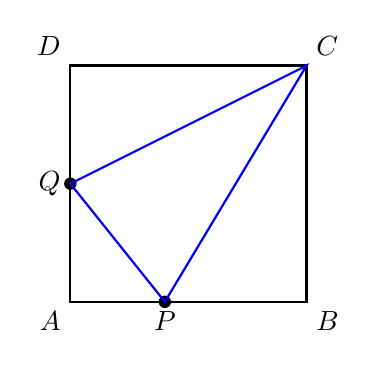
\begin{tikzpicture}[scale=1.5]
\draw[thick] (0,0) rectangle (2,2);
\node[below left] at (0,0) {$A$};
\node[below right] at (2,0) {$B$};
\node[above right] at (2,2) {$C$};
\node[above left] at (0,2) {$D$};
\fill (0.8,0) circle (1.5pt); \node[below] at (0.8,0) {$P$};
\fill (0,1.0) circle (1.5pt); \node[left] at (0,1.0) {$Q$};
\draw[thick,blue] (0,1.0) -- (2,2) -- (0.8,0) -- (0,1.0);
\end{tikzpicture}
\end{center}
\end{frame}

\begin{frame}[t]{第23题 解答}
\begin{tcolorbox}[colback=orange!10,colframe=orange,title=\textbf{解}]
设 $AP=x$，$AQ=y$，则 $PQ=\sqrt{x^2+y^2}$。
由周长 $x+y+\sqrt{x^2+y^2}=2$，得 $\sqrt{x^2+y^2}=2-x-y$。平方：$x^2+y^2=4+x^2+y^2+2xy-4x-4y$，即 $2xy-4x-4y+4=0$，$xy-2x-2y+2=0$。

设 $\angle BCP=\alpha$，$\angle DCQ=\beta$，则 $\tan\alpha=\dfrac{PB}{BC}=1-x$，$\tan\beta=1-y$。
\[
\tan(\alpha+\beta)=\frac{(1-x)+(1-y)}{1-(1-x)(1-y)}=\frac{2-x-y}{x+y-xy}.
\]
由 $xy=2x+2y-2$，分母 $=x+y-(2x+2y-2)=2-x-y$。
故 $\tan(\alpha+\beta)=1$。又 $\alpha+\beta\in(0,\frac{\pi}{2})$，$\alpha+\beta=\dfrac{\pi}{4}$。
$\angle PCQ=\dfrac{\pi}{2}-(\alpha+\beta)=\dfrac{\pi}{4}$。
\end{tcolorbox}
\end{frame}

% ===== 拓广探索 =====
\begin{frame}{第三部分：拓广探索（第24--27题）}
\end{frame}

% --- 24 ---
\begin{frame}[t]{第24题：由 $\sin\beta+\cos\beta=\frac15$}
\textbf{24.} 已知 $\sin\beta+\cos\beta=\dfrac15$，$\beta\in(0,\pi)$。
\begin{enumerate}
  \item 求 $\tan\beta$ 的值；
  \item 你能根据所给的条件，自己构造出一些求值问题吗？
\end{enumerate}
\end{frame}

\begin{frame}[t]{第24题 解答}
\begin{tcolorbox}[colback=orange!10,colframe=orange,title=\textbf{解}]
平方：$1+\sin 2\beta=\dfrac1{25}$，$\sin 2\beta=-\dfrac{24}{25}<0$。
$\beta\in(0,\pi)$，故 $\beta\in(\frac{\pi}{2},\pi)$，$\sin\beta>0,\cos\beta<0$。
$(\sin\beta-\cos\beta)^2=1-\sin 2\beta=\dfrac{49}{25}$，$\sin\beta-\cos\beta=\dfrac75$。
与 $\sin\beta+\cos\beta=\dfrac15$ 联立：$\sin\beta=\dfrac45$，$\cos\beta=-\dfrac35$。
\alert{$\tan\beta=-\dfrac43$}。
\end{tcolorbox}
\end{frame}

% --- 25 ---
\begin{frame}[t]{第25题：平行线间的三角形面积}
\textbf{25.} 直线 $l_1\parallel l_2$，$A$ 是 $l_1,l_2$ 之间定点，$A$ 到 $l_1,l_2$ 距离分别为 $h_1,h_2$。$B$ 是 $l_2$ 上动点，作 $AC\perp AB$ 交 $l_1$ 于 $C$，设 $\angle ABD=\alpha$。
\begin{enumerate}
  \item 写出 $\triangle ABC$ 面积 $S$ 关于 $\alpha$ 的解析式 $S(\alpha)$；
  \item 画出上述函数图象；
  \item 由图象求 $S(\alpha)$ 的最小值。
\end{enumerate}
\end{frame}

\begin{frame}[t]{第25题 解答}
\begin{tcolorbox}[colback=orange!10,colframe=orange,title=\textbf{解}]
在 $\text{Rt}\triangle ABD$ 中（$D$ 为 $A$ 在 $l_2$ 上垂足），$AB=\dfrac{h_2}{\sin\alpha}$。
$\angle BAC=90^\circ$，故 $\angle EAC=\alpha$（$E$ 为 $A$ 在 $l_1$ 上垂足），$AC=\dfrac{h_1}{\cos\alpha}$。
因 $AB\perp AC$：
\[
S(\alpha)=\frac12 AB\cdot AC=\frac{h_1h_2}{2\sin\alpha\cos\alpha}=\frac{h_1h_2}{\sin 2\alpha}.
\]
当 $\sin 2\alpha=1$ 即 $\alpha=\dfrac{\pi}{4}$ 时，$S_{\min}=h_1h_2$。
\end{tcolorbox}
\end{frame}

% --- 26 ---
\begin{frame}[t]{第26题：泰勒展开}
\textbf{26.} 英国数学家泰勒给出公式：
\[
\sin x=x-\frac{x^3}{3!}+\frac{x^5}{5!}-\frac{x^7}{7!}+\cdots,\qquad
\cos x=1-\frac{x^2}{2!}+\frac{x^4}{4!}-\frac{x^6}{6!}+\cdots.
\]
试用计算工具计算 $\cos 0.3$，并与前三项近似 $1-\dfrac{0.3^2}{2!}+\dfrac{0.3^4}{4!}=0.9553375$ 比较。
\end{frame}

\begin{frame}[t]{第26题 解答}
\begin{tcolorbox}[colback=orange!10,colframe=orange,title=\textbf{解}]
精确计算 $\cos 0.3\approx 0.9553365$。
前三项近似值 $0.9553375$，误差约 $10^{-6}$，精度已非常高。
这说明泰勒级数在 $|x|$ 较小时收敛很快，前几项即可满足工程精度。
\end{tcolorbox}
\end{frame}

% --- 27 ---
\begin{frame}[t]{第27题：太阳直射点纬度}
\textbf{27.} 地球公转中太阳直射点纬度随时间周而复始。正午太阳高度角 $\theta$、直射点纬度 $\delta$、当地纬度 $\varphi$ 满足 $\theta=90^\circ-|\varphi-\delta|$。某科技小组以春分（直射赤道）为初始时刻，统计连续 $400$ 天直射点纬度平均值 $y$。三处观测站春分后第 $45$ 天测得：

\begin{center}
\begin{tabular}{|l|c|c|c|}
\hline
 & A & B & C\\
\hline
观测站纬度 $\varphi$ / 度 & $40.0000$ & $23.4393$ & $0.0000$\\
正午太阳高度角 $\theta$ / 度 & $66.3870$ & $82.9464$ & $73.6141$\\
\hline
\end{tabular}
\end{center}
(1) 完成表格（求 $\delta$）；(2) 设 $y=A\sin\omega x$，$A=23.4392911^\circ$，估计 $\omega$；(3) 求回归年天数；(4) 估计 $400$ 年中闰年个数。
\end{frame}

\begin{frame}[t]{第27题 解答}
\begin{tcolorbox}[colback=orange!10,colframe=orange,title=\textbf{解}]
(1) 由 $\delta=\varphi-(90^\circ-\theta)$（春分后直射点北移，$\delta>0$）：
A：$\delta=40.0000-(90-66.3870)=16.3870^\circ$；
B：$\delta=23.4393-(90-82.9464)=16.3857^\circ$；
C：$\delta=0-(90-73.6141)=16.3859^\circ$。

(2) $x=45$，$y\approx 16.386^\circ$，$A=23.4393^\circ$：$\sin(45\omega)=16.386/23.4393\approx 0.6991$，$45\omega\approx 0.774^\circ$（弧度），$\omega\approx 0.0172$ rad/天。

(3) 回归年 $T=\dfrac{2\pi}{\omega}\approx 365.242$ 天。

(4) $400$ 年总天数 $400\times 365.242=146096.8$，$400$ 个平年共 $146000$ 天，需补 $96.8\approx 97$ 个闰年（现行公历 $400$ 年 $97$ 闰）。
\end{tcolorbox}
\end{frame}

\begin{frame}[c]
  \begin{center}
    {\Huge\calligra Thanks!}
  \end{center}
\end{frame}

\end{document}
